\documentclass{article}
\usepackage[utf8]{inputenc}
\usepackage{hyperref}
\usepackage{url}
\usepackage{mathtools}
\usepackage{amsmath}
\usepackage{graphicx}
\usepackage{wrapfig}
\usepackage{algorithm}
\usepackage{algpseudocode}
\usepackage{subcaption}
\usepackage[svgnames]{xcolor}
\usepackage{listings}
\usepackage[left=2.5cm, right=2.5cm, top=1.5cm, bottom=2cm]{geometry}
\setcounter{section}{-1}


\title{
\textbf{Algorithmics for Data Mining: Deliverable 3\\} \Large{
    Democrat Vs. Republican Tweets}}
\author{Oriol Borrell\\
\textit{\small FIB - UPC Student} \\
\textit{\small Barcelona, Spain} \\
\textit{\texttt{\href{mailto:oriol.borrell.roig@est.fib.upc.edu}
{\small oriol.borrell.roig@est.fib.upc.edu}}}}
\date{\today}

\begin{document}
\maketitle

\section{Abstract}

\textit{
We will analyze what do politicians of the Republican and Democrat Parties (in USA) tweet about. We will first see if we can extract any conclusion about particularities of each party tweet. Afterwords we will train a model that will predict, given a tweet, if it belongs to the Republican or to the Democrat party.
}

\section{Context}
\label{Context}
The tweets obtained are all tweet from 2019 of USA politician's. We have to take into account that Donald Trump (from the Republican party) is the president of USA since January 20, 2017. The Democrat's candidate was Hillary Clinton. The 2019 in USA was a Off-year election.

Republicans and Democrats are the two main and historically the largest political parties in the US. After every election, they hold the majority seats in the House of Representatives and the Senate as well as the highest number of Governors.

\section{What do Democrat and Republican members tweet about?}

Before analyze the tweets we applied the following preprocessing steps:
\begin{itemize}
    \item Remove the newline characters
    \item Remove commonly used ampersand
    \item Remove ' from contractions such as I'm and don't
    \item Lowercase the string
    \item Remove https-links from the string
    \item Tokenize the string with the given pattern
\end{itemize}

Once we had the tokens, we computed the frequencies of each token in each party. We created the wordcloud shown in Figure \ref{fig:WordCloud100}.

\begin{figure}[H]
    \centering
    \begin{subfigure}{.8\textwidth}
        \centering
        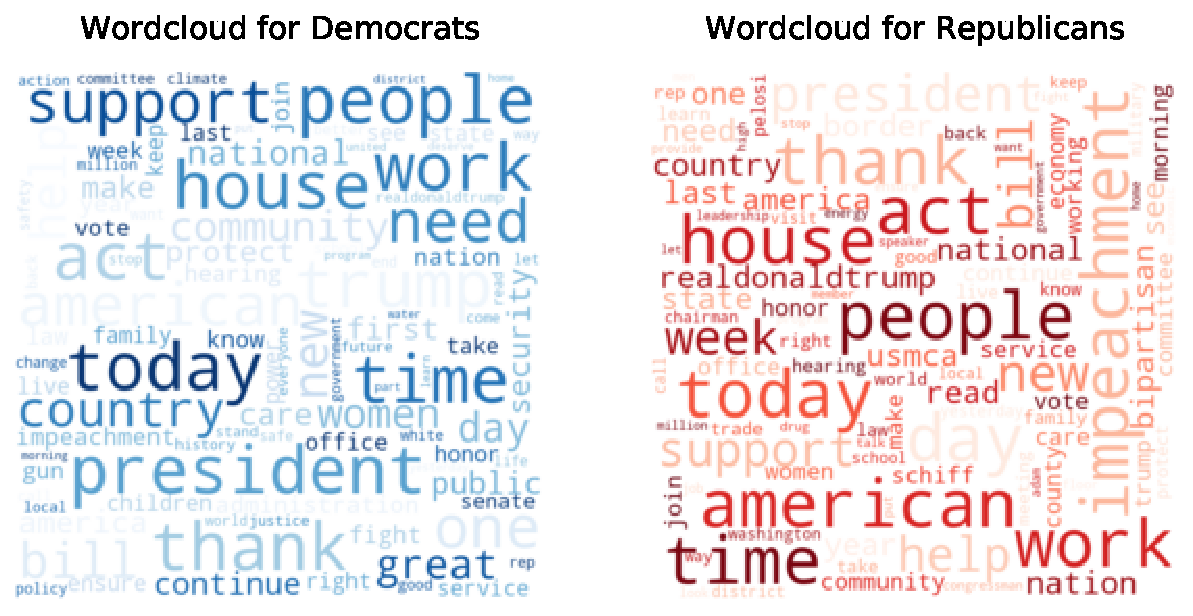
\includegraphics[width=1\textwidth]{./img/WordCloud100.pdf}
    \end{subfigure}
    \caption{Wordcloud of the top used tokens of each party}
    \label{fig:WordCloud100}
\end{figure}

Analyzing the results, we observe that the most used words of each party are fairly common words in the field of politicsWe cannot extract any particularity neither from the Democrats nor Republicans.

Doing a bit of research I founded a common concept in \textit{Information Retival} called Term Frequency–Inverse Document Frequency, \textbf{TFIDF}. TFIIDF is a way to compute the importance a word is in a document. As shown in Equation \ref{eq:TFIDF} is computed using two statics, the \textit{Term Frequency(tf)}, and the \textit{Inverse document frequency(idf)}:

\begin{equation} \label{eq:TFIDF}
    \begin{split}
        & tf(t,d) = 0.5 + 0.5\times \frac{f_{t,d}}{max\{f_{t^{'},d}: t^{'} \in d\}} \\
        & idf(t,D) = log \frac{N}{|d\in D:t\in d|} \\ \\
        & tfidf(t,d,D)  = tf(t,d)\times idf(t,D) 
    \end{split}
\end{equation}

Where $f_{t,d}$ is the frequency of the token \textit{t} in the document \textit{d}, and $N$ is the total number of documents in the collection.

Once we computed the TFIDF, we created another time the wordcloud of each party. The results are shown in Figure \ref{fig:WordCloudTFIDF}

\begin{figure}[H]
    \centering
    \begin{subfigure}{.8\textwidth}
        \centering
        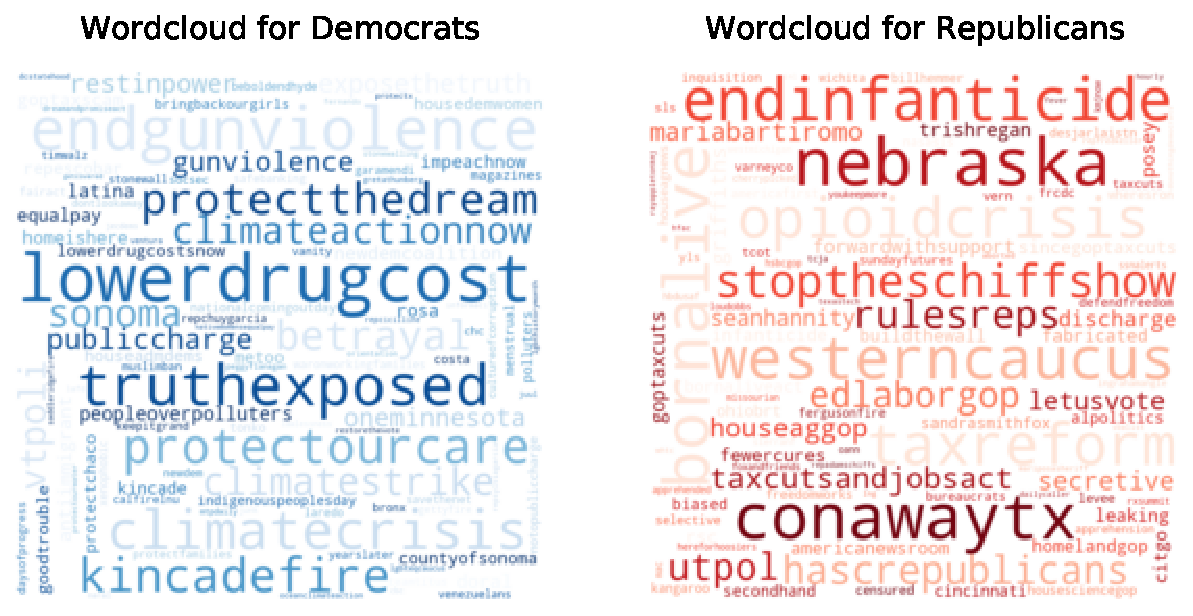
\includegraphics[width=1\textwidth]{./img/WordCloudTFIDF.pdf}
    \end{subfigure}
    \caption{Wordcloud using TFIDF}
    \label{fig:WordCloudTFIDF}
\end{figure}


The obtained wordclouds are very interesting. We see that the Democrats apparently have a larger focus on \textit{climate} and \textit{health care} where the Republicans focus on \textit{anti-abortion} and \textit{tax-cuts}. These topics are all more interesting and polarizing than the previous results, where we saw that both parties often referred to different political personalities, committees and other political jargon. We see a clear indicator, that the phrases for both parties are political slogans, such as \textit{endgunviolence} and \textit{bornalive}. Twitter, therefore, gives us a valuable insight into the key-issues and focal points of each party.

\section{Convolutional Neural Networks (CNN)}
\label{CNN}

A Convolutional Neural Network (CNN) is a specific type of artificial neural network that has some hidden layers called convolutional layers, where the transformation is made in this layer is a convolutional operation. CNNs is widely used to do image recognition, image classifications, objects detections, faces recognition etc., that's the reason I choosed this algorithm.

The model type that was used was Sequential. It allows you to build a model layer by layer. In our model we will use the following type of layers:

\begin{itemize}
    \item \textbf{Conv2D:} This layer creates a convolution kernel that is convolved with the layer input to produce a tensor of outputs.
    \item \textbf{MaxPool2D:} Takes the maximum value of the kernel to reduce the number of parameters.
    \item \textbf{SpatialDropout2D:} We randomly set entire kernel to 0. So we will drop them, in order to prevent for overfiting.
    \item \textbf{Flatten:} It reduces the dimension of the data into 1 dimension.
    \item \textbf{Dropout:}It randomly turn off neurons in order to reduce overfitting.
    \item \textbf{Dense:} We take the dimension created in the flattern layer and convert it into the category to predict.
    
\end{itemize}
 
The following table shows the CNN i designed:

\begin{table}[ht]
    \centering
    \begin{tabular}{|l|ccc|}
        \hline
        \textbf{Layer(type)} & \textbf{Units} & \textbf{Filter} & \textbf{Stride} \\
        \hline
        Conv2D & 8 & 5 & 2 \\ \hline
        Conv2D & 32 & 3 & 1\\ \hline
        MaxPool2D & - & 3 & 2\\ \hline
        SpatialDropout2D & - & - & -\\ \hline

        Conv2D & 64 & 3 & 2\\ \hline
        Conv2D & 64 & 3 & 1\\ \hline
        MaxPool2D & - & 3 & 2\\ \hline
        SpatialDropout2D & - & - & -\\ \hline

        Conv2D & 128 & 1 & 1\\ \hline
        Conv2D & 128 & 1 & 1\\ \hline
        Conv2D & 128 & 1 & 1\\ \hline
        SpatialDropout2D & - & - & -\\ \hline

        Flatten & - & - & -\\ \hline
        Dropout & - & - & -\\ \hline
        Dense & 5 & - & -\\ \hline

    \end{tabular}
    \caption{Accuracy obtained respect $k$}
    \label{tab:knn_results}
\end{table}

When we built the model we tried allot of possibles parametritzations for the number of nodes in each Conv2D layer. Finaly, in the first set of layers we have 8 nodes, and 32, tn the second one two layers of 64 nodes, and in the third one three layers of 128 nodes. This are the number of nodes that made us reach the higher accuracy. Another parametrization we choosed was the kernel size, the size of the filter matrix for our convolution. We decided to create $3 \times 3$ size filter matrix, except in the first layer, that will be a $5 \times 5$ matrix, and in the last set of Conv2D layers.

We also had to define the number of \textit{epochs} (number of times we train the model with the same training/testing data) we will perform. If we set a low number of epochs our model could not be enough trained. If we set a big number of epochs, our model could be overfitted. In both cases the accuracy will decrease, so the number of epochs important.

So we first built the model with 50 epochs, and plotted the acuracy and lost values of each one. In Figures \ref{fig:EpochAccuracy} and \ref{fig:EpochLoss} we can clearly see that after epoch 15 we have a overfitted model, as is when in both figures the train and test lines are starting to take different directions. So we rebuilt the model with 15 epochs.

With all this parametritzations, once built the model we validated with the data saved for that purpose. We obtained an accuracy of \textbf{0.8373}. With this model we can be much more confident of our prediction in comparison to $k$-NN. We have to take into account that CNN is a neural network, and this works well with huge amount of data. So is probable that if we train the model with much more data, the accuracy will be higher.

\section{Evaluation do the results}

The results obtained with a KNN clasifier gave us an improvement comparing it with "flipping a coin" to predict the category. However, the accuracy obtained is not the one that we expected.  Comparing the two models we created, for this project we would clearly choose the CNN one. The best parametrization we found for the CNN gave us a 0.8373 of accuracy, which we conclude that is an acceptable result for this project. 

However, the important thing of this project was not only to obtain a high accuracy, but also to learn the different parts of a CNN and to detect overfitting. We also can affirm that we completed this goal of the project.

\section{Implementation}
In order to play a little with the model we built, just for fun, we drew som images using the paint application for windows operating systems. We used our model to predict the their category. The images created are the ones shown in Figure \ref{fig:PaintDrawings}:


The Table shows the obtained predictions. Each column represents a image (each letter refers to the letters assigned in Figure \ref{fig:PaintDrawings}). Each row represents the probability the model said of being for a certain category:

\begin{table}[ht]
    \centering
    \begin{tabular}{|l|cccccc|}
        \hline
        \textbf{Category} & \textbf{a} & \textbf{b} & \textbf{c} & \textbf{d} & \textbf{e} & \textbf{f} \\
        \hline
        Ambulance           & 0.00\% & 0.05\% & 0.12\% & 0.00\% & 100.00\% & 0.00\%   \\ \hline
        Angel               & 0.00\% & 0.00\% & 0.00\% & 99.97\% & 0.00\% & 0.00\% \\ \hline
        Aircraft carrier    & 1.49\% & 99.85\% & 12.67\% & 0.00\% & 0.00\% & 0.00\%  \\ \hline
        Airplane            & 98.51\% & 0.08\% & 84.13\% & 0.00\% & 0.00\% & 0.00\%  \\ \hline
        Ant                 & 0.00\% & 0.02\% & 3.07\% & 0.03\% & 0.00\% & 100.00\%  \\ \hline

    \end{tabular}
    \caption{Accuracy obtained respect $k$}
    \label{tab:knn_results}
\end{table}


\end{document}
